\documentclass[12pt, a4]{article}
\usepackage[english]{babel}
\usepackage[utf8x]{inputenc}
\usepackage{fullpage}
\usepackage{listings}
\usepackage{graphicx}
\usepackage{color}

%Syntax highlighting
\definecolor{blue-violet}{rgb}{0.54, 0.17, 0.89}
\definecolor{ao}{rgb}{0.0, 0.5, 0.0}
\definecolor{amaranth}{rgb}{0.9, 0.17, 0.31}
\definecolor{ballblue}{rgb}{0.13, 0.67, 0.8}
\definecolor{onyx}{rgb}{0.06, 0.06, 0.06}


\lstset{
  breaklines=true,                 % automatic line breaking only at whitespace
  captionpos=b,                    % sets the caption-position to bottom
  breakatwhitespace=false,
  keepspaces=true,
  numbers=left,
  numbersep=5pt,
  showspaces=false,
  showstringspaces=false,
  showtabs=false,
  tabsize=4,  
  backgroundcolor=\color{white},   % choose the background color
  commentstyle=\color{ao},    % comment style
  keywordstyle=\color{amaranth},    % keyword style
  stringstyle=\color{blue-violet},    % string literal style
  numberstyle=\tiny\color{ballblue},	   % number style
  basicstyle=\ttfamily\footnotesize\color{onyx} % size of fonts used for the code
}

%Document Header
\title{\textbf{Department of CSE\\SSN College of Engineering}}
\author{\textbf{Vishakan Subramanian - 18 5001 196 - Semester VII}}
\date{03 October 2021}

\begin{document}
\maketitle
\hrule
\section*{\center{UCS 1711 - Mobile Application Development Lab}}
\hrule
\bigskip

%Assignment Details
\subsection*{\center{\textbf{Exercise 6: GPS Location Application}}}
\subsection*{\flushleft{Aim:}}
\begin{flushleft}

To develop a native application that makes use of GPS location information.

\end{flushleft}

%Code
\newpage
\subsection*{\flushleft{Code - GPS Location: Main Activity:}}
\begin{flushleft}
\lstinputlisting[language = Java]{GPS/app/src/main/java/com/example/gps/MainActivity.java}
\end{flushleft}

%Code
\newpage
\subsection*{\flushleft{Code - GPS Location: Main Activity Layout:}}
\begin{flushleft}
\lstinputlisting[language = XML]{GPS/app/src/main/res/layout/activity_main.xml}
\end{flushleft}

%Code
\newpage
\subsection*{\flushleft{Code - GPS Location: Android Manifest XML:}}
\begin{flushleft}
\lstinputlisting[language = XML]{GPS/app/src/main/AndroidManifest.xml}
\end{flushleft}


%Output
\newpage
\subsection*{\flushleft{Output: Location Permission:}}
\begin{figure}[h]
\centering
\caption{Output: Location Permission.}
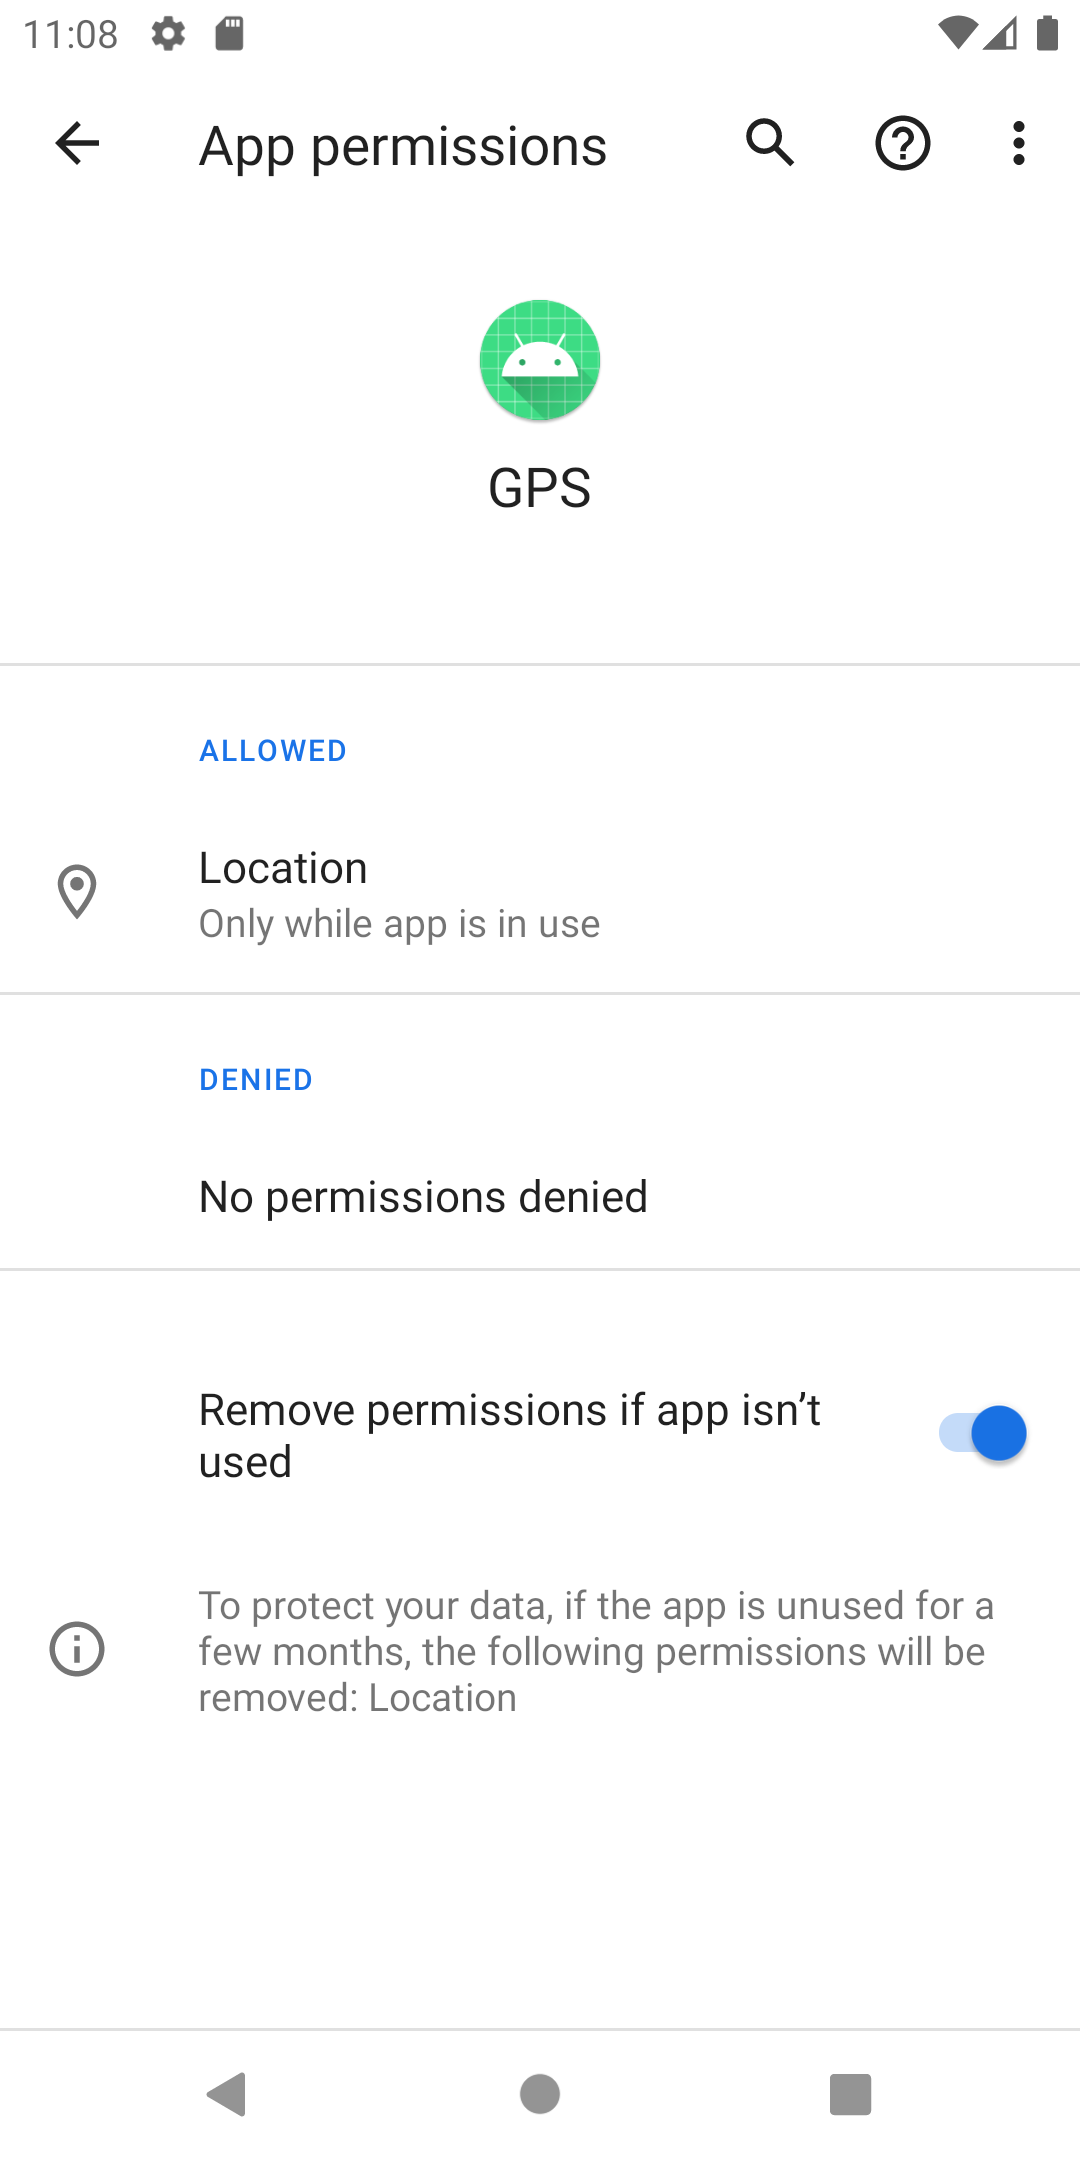
\includegraphics[height=15cm, width=7.3cm]{GPS/Screenshots/Output-0.png}
\end{figure}

%Output
\newpage
\subsection*{\flushleft{Output: GPS Location:}}
\begin{figure}[h]
\centering
\caption{Output: GPS Location.}
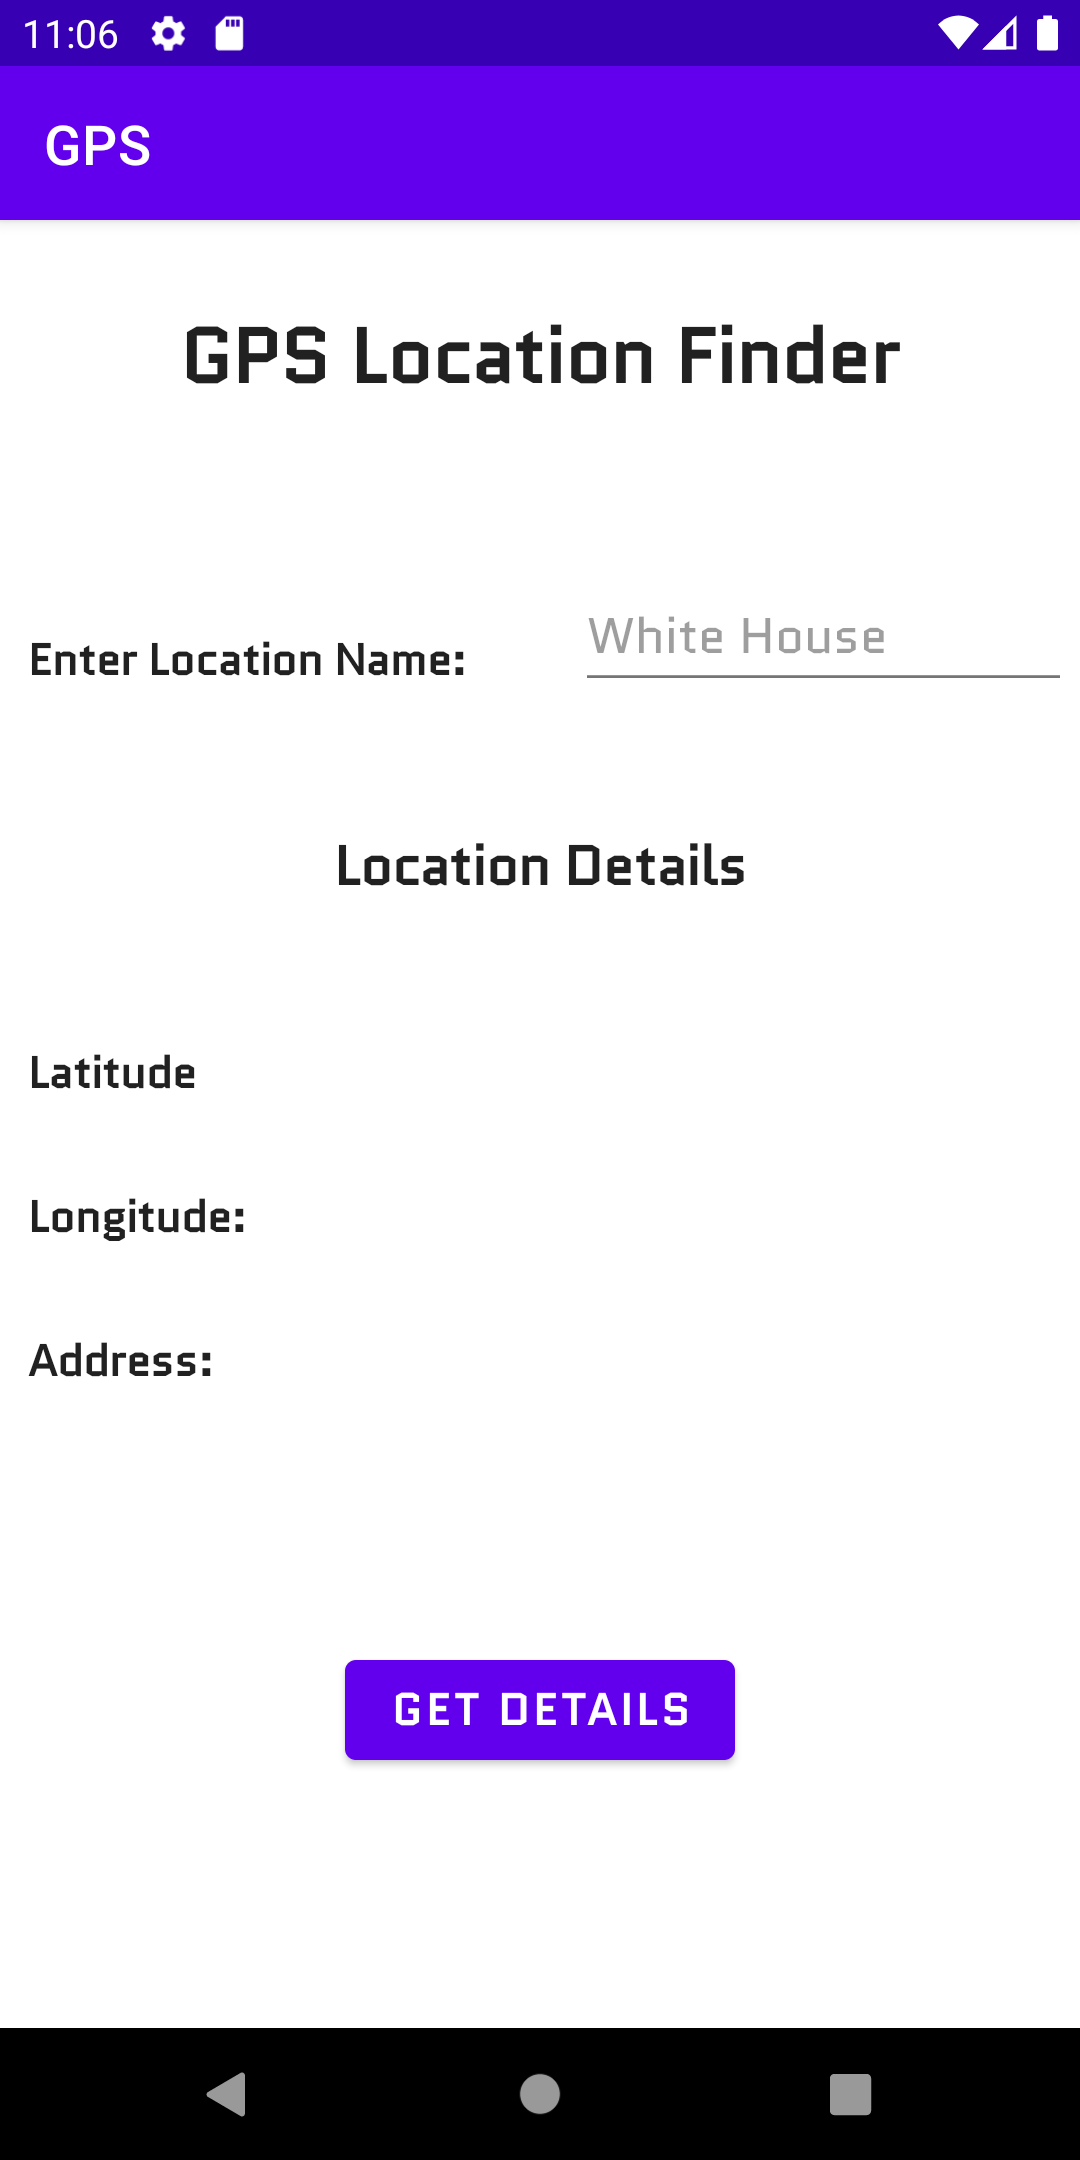
\includegraphics[height=15cm, width=7.3cm]{GPS/Screenshots/Output-1.png}
\end{figure}

%Output
\newpage
\subsection*{\flushleft{Output: GPS Location - SSN College:}}
\begin{figure}[h]
\centering
\caption{Output: GPS Location - SSN College.}
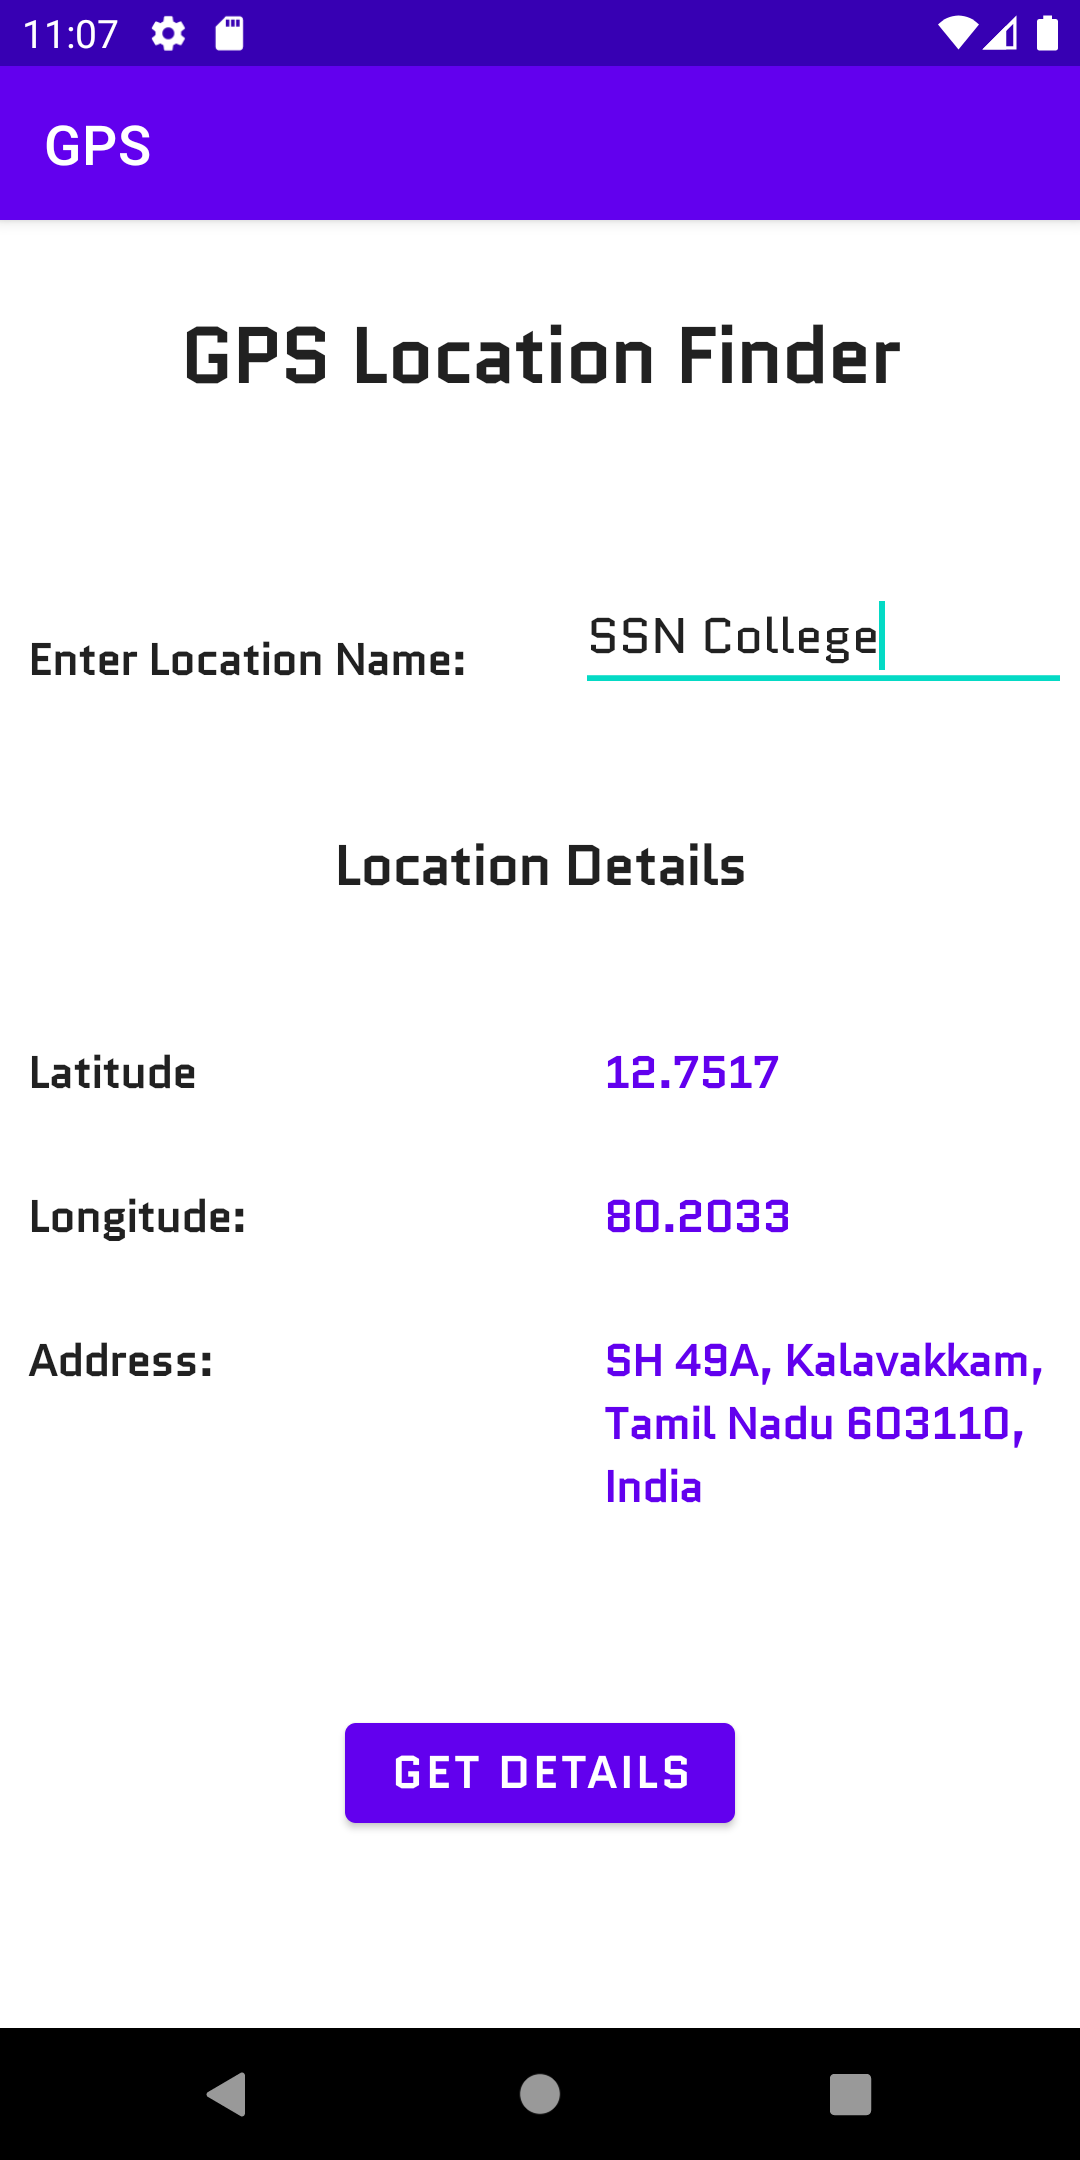
\includegraphics[height=15cm, width=7.3cm]{GPS/Screenshots/Output-2.png}
\end{figure}


%Learning Outcome
\newpage
\subsection*{\flushleft{Learning Outcome:}}
\begin{itemize}

\item I learnt how to set application permissions for 
\textbf{COARSE LOCATION, FINE LOCATION \& INTERNET} using the AndroidManifest.xml file.
\item I implemented conditions to check whether location permissions have been granted for the application.
\item I learnt about \textbf{Geocoder} and its relevant method \textbf{getFromLocationName()} to get \textbf{Address} details of a particular place.
\item I used the \textbf{Address} object to retrieve details like \textbf{latitude, longitude \& street address}.
\item I displayed the appropriate GPS results to the user via the UI. 
\item I was also able to handle error cases wherein the requested location was not found with the use of the Geocoder methods.

\end{itemize}


\end{document}